\documentclass[letterpaper,spanish,10pt]{article}
\usepackage[latin1]{inputenc}    % Agregar y acentos
\usepackage{babel}               % Soporte multilenguajes
\usepackage{avant}               % Tipo de fuente
%\usepackage{fancyheadings}      % Topes y pies de p'agina
\usepackage[dvips]{graphicx}     % Inclusion de imagenes .eps
\usepackage{url}                 % Agregar Links soporte de ~
\usepackage{verbatim}
\usepackage{geometry}
\usepackage{url}
\usepackage{amsfonts}
\usepackage{amssymb}
%\usepackage{txfonts}
%\usepackage{emphoff}
%\usepackage{pxfonts}
%\usepackage{fancybox}
\usepackage{latexsym}
%\usepackage{fancyvrb}
\usepackage{graphicx}
%\usepackage{wasysym}
%\renewcommand{\baselinestretch}{1.5}
\parskip=7mm
\pagestyle{myheadings}
\geometry{tmargin=4cm, bmargin=4cm, lmargin=2.5cm, rmargin=2.5cm}
\markright{\hrulefill Proyecto Hevelius $\; \;$}


%opening
\title{{\Huge \bf Proyecto Hevelius} \\ {\Large Empresa DevNull} \\ {\small Plan de Proyecto}}

\author{
{\bf Carlos Guajardo Miranda} \\ Jefe de Proyecto \\ \url{cguajard@alumnos.inf.utfsm.cl} \\ cel. 09-95046118 
\and
{\bf Marina Pilar Daza} \\ Miembro del Equipo \\ \url{mpilar@alumnos.inf.utfsm.cl} \\ cel. 09-84085407
\and
{\bf Esteban Espinoza Mart\'inez} \\ Miembro del Equipo \\ \url{eespinoz@alumnos.inf.utfsm.cl} \\ cel. 09-85596939
\and
{\bf Tom\'as Staig Fern\'andez} \\ Miembro del Equipo \\ \url{tstaig@alumnos.inf.utfsm.cl} \\ cel. 09-97615666
}


\date{25 de mayo de 2007}


\begin{document}

% Portada
\maketitle
\newpage

% Indices
\tableofcontents{}
\newpage




\section{Introducci\'on}
En el presente documento se da a conocer el plan del Proyecto Hevelius, el cual 
tiene por objetivo mostrar el estudio realizado por la Empresa DevNull. 
En este estudio se contemplan las soluciones al desaf\'io planteado por el grupo
ACS-UTFSM, as\'i como la concretitud de los requerimientos de \'estos.

Se advierte que el car\'acter t\'ecnico, desarrollado en algunos \'items del documento,
est\'a dirigido a discusiones concretas y son comprensibles por el grupo ACS-UTFSM 
y por personas vinculadas con el tema.

El documento se estructura de la siguiente forma:
\begin{itemize}
        \item \textbf{Soluci\'on conceptual:} En la cual se describe el problema 
actual, se bosquejan posibles soluciones y, finalmente, se escoge la mejor alternativa.
        \item \textbf{T\'ecnicas y herramientas de desarrollo:} Esto es, definir 
los elementos t\'ecnicos con que se construir\'a la soluci\'on y la plantilla de trabajo.
        \item \textbf{Gesti\'on de riesgos:} En esta secci\'on se identificar\'an, 
clasificar\'an y se propondr\'an estrategias de mitigaci\'on y contingencia para los 
peligros ocurrentes del proyecto.
        \item \textbf{Implementaci\'on:} En la cual se explica la incorporaci\'on del 
nuevo sistema en las instalaciones del cliente.
        \item \textbf{Planificaci\'on de actividades:} Esto significa describir el 
proceso que se seguir\'a para llevar a cabo la soluci\'on propuesta.
\end{itemize}

En el contexto m\'as general, el desaf\'io planteado por el grupo ACS-UTFSM, es 
crear un sistema de control de telescipios capaz de poder manejar cualquier telescopio 
que se conecte a trav\'es de las diferentes coordenadas utilizadas en el mundo 
astron\'omico.\\

Lo que se espera crear consiste en una interfaz gr\'afica que permita operar al 
alg\'un telescopio de manera remota, lograr un control en tiempo real y generar 
registros para posteriores an\'alisis de los datos recibidos por el telescopio.\\

La mejor soluci\'on ideada, es el dise\~no y construcci\'on de un producto de software dise\~nado 
para solventar los problemas actuales y cumplir con los requerimientos del cliente.\\

Los riesgos, que se detallan en el cap\'itulo 4, corresponden a los peligros identificados 
que pueden aparecer durante el desarrollo del proyecto, entre ellos se destaca: la poca 
escalabilidad del sistema de control y el no cumplimiento de los est\'andares ALMA.




\newpage
\section{Soluci\'on Conceptual} %%% TOMAS
\subsection{Diagn\'ostico de la situaci\'on actual}
\subsubsection{Situaci\'on Actual}

Los telescopios son una herramienta fundamental para la astronom\'ia, cada
perfeccionamiento del telescopio ha sido seguido de avances en la comprensi\'on 
del universo.
Existen varios tipos de telescopio, notablemente refractores, que utilizan 
lentes, reflectores, que tienen un espejo c\'oncavo en lugar de la lente del
 objetivo, y catadi\'optricos, que poseen un espejo c\'oncavo y una lente correctora.

El par\'ametro m\'as importante de un telescopio es el di\'ametro de su objetivo. 
Un telescopio de aficionado generalmente tiene entre 76 y 150 mm de di\'ametro y 
permite observar algunos detalles planetarios y much\'isimos objetos del cielo 
profundo (c\'umulos, nebulosas y algunas galaxias). Los telescopios que superan  
los 0,20 m de di\'ametro permiten ver detalles lunares finos, detalles planetarios 
importantes y una gran cantidad de c\'umulos, nebulosas y galaxias brillantes 
y que se encuentran implementados en los observatorios.

Para caracterizar un telescopio y utilizarlo se emplean una serie de par\'ametros y accesorios:
\begin{itemize}
    \item Distancia Focal: es la longitud focal del telescopio, pero se define como la distancia del espejo principal hasta el final del tubo.
    \item Di\'ametro del objetivo: Di\'ametro del espejo o lente primaria del telescopio.
    \item Ocular: Accesorio peque\~no que colocado en el foco del telescopio permite magnificar la imagen de los objetos.
    \item Lente de Barlow: Lente que generalmente duplica o triplica los aumentos del ocular cuando se observan los astros.
    \item Filtro: peque\~no accesorio que generalmente opaca la imagen del astro pero que dependiendo de su color y material suele ser beneficioso y se ubica delante del ocular.
    \item Raz\'on Focal: es el cociente entre la distancia focal (mm) y el di\'ametro (mm). (f/ratio)
    \item Magnitud l\'imite: es la magnitud m\'axima que se puede ver en un lugar dado, es decir, el brillo de la estrella m\'as d\'ebil visible.
    \item Tr\'ipode: Conjunto de tres patas generalmente de aluminio que le dan soporte y estabilidad al telescopio.
    \item Portaocular: Orificio d\'onde se colocan el ocular y la lente de Barlow.
\end{itemize}

Como se puede apreciar los componentes de los telescopios son bastante complejos, 
pero m\'as a\'un cuando se quiere obtener la ubicaci\'on de alguna estrella u objeto 
celeste, ya que no es s\'olo dar coordenadas, porque tanto el objeto a observar como 
nuestro punto base(la tierra) se mueven de distintas formas, debido a que durante el 
transcurso de un d\'ia, la Tierra se habr\'a movido un poco a lo largo de su \'orbita 
alrededor del Sol, por lo que debe girar una peque\~na distancia angular extra antes 
de que el Sol alcance su punto m\'as alto. En cambio las estrellas est\'an tan alejadas 
que el movimiento de la Tierra a lo largo de su \'orbita genera una diferencia apenas 
apreciable con respecto a su direcci\'on aparente, por lo que vuelven a su punto m\'as 
alto en algo menos de 24 horas o d\'ia solar. Una idea de esta situaci\'on es la siguiente:
\begin{figure}[h!]
 \centering
 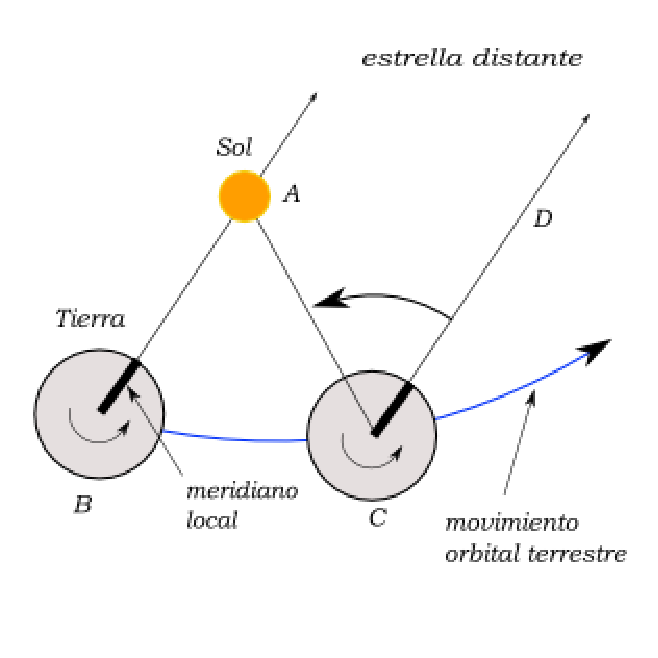
\includegraphics[scale=0.7]{tmp.eps}
 \caption{Situaci\'on estrella-tierra}
 %\label{fig:yeti}
\end{figure} 

Por lo que existen sistemas de coordenadas especiales como son Sistema de coordenadas 
Horizontales, Ecuatoriales, Ecl\'ipticas, entre otras, para poder simplificar 
esta situaci\'on. Estos sistemas de coordenadas usan como referencia la hora actual, 
ubicaci\'on geogr\'afica y otros factores para realizar las conversiones entre ellas.
 Adem\'as de estas condiciones existe una gran cantidad de cosas que afectan el poder
realizar este tipos de observaciones, como son la luz solar, que da\~na los telescopios, 
algunas condiciones clim\'aticas, la luminosidad de la luna, entre otras cosas, lo que 
hace que los operadores de telescopios est\'en sumamente atentos a estos importantes 
acontecimientos que pueden da\~nar gravemente el telescopio. Actualmente existen
c\'upulas para los telescopios que tienen la funci\'on de proteger el telescopio y 
la instrumentaci\'on cient\'ifica, al tiempo que sigue sus movimientos y le permite 
explorar la b\'oveda celeste.
\newpage
\begin{figure}[h!]
 \centering
 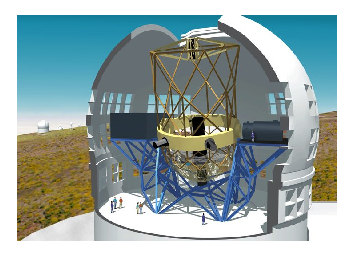
\includegraphics[scale=1.5]{cup.eps}
 \caption{C\'upula que protege el telescopio}
 %\label{fig:yeti}
\end{figure}

Despu\'es de esta peque\~na descripci\'on podemos apreciar que para poder manejar 
un telescopio se necesitan d\'ias de preparaci\'on antes de poder trabajar con 
\'el, ya que sus interfaces son complicadas y muy detalladas y para cada telescopio 
existe una interfaz distinta, implementada de diferente forma, dependiendo del lugar
en donde se cre\'o, por esto mismo, puede estar en diversos idiomas. Un ejemplo de 
una interfaz es la que se muestra a continuaci\'on:

\begin{figure}[h!]
 \centering
 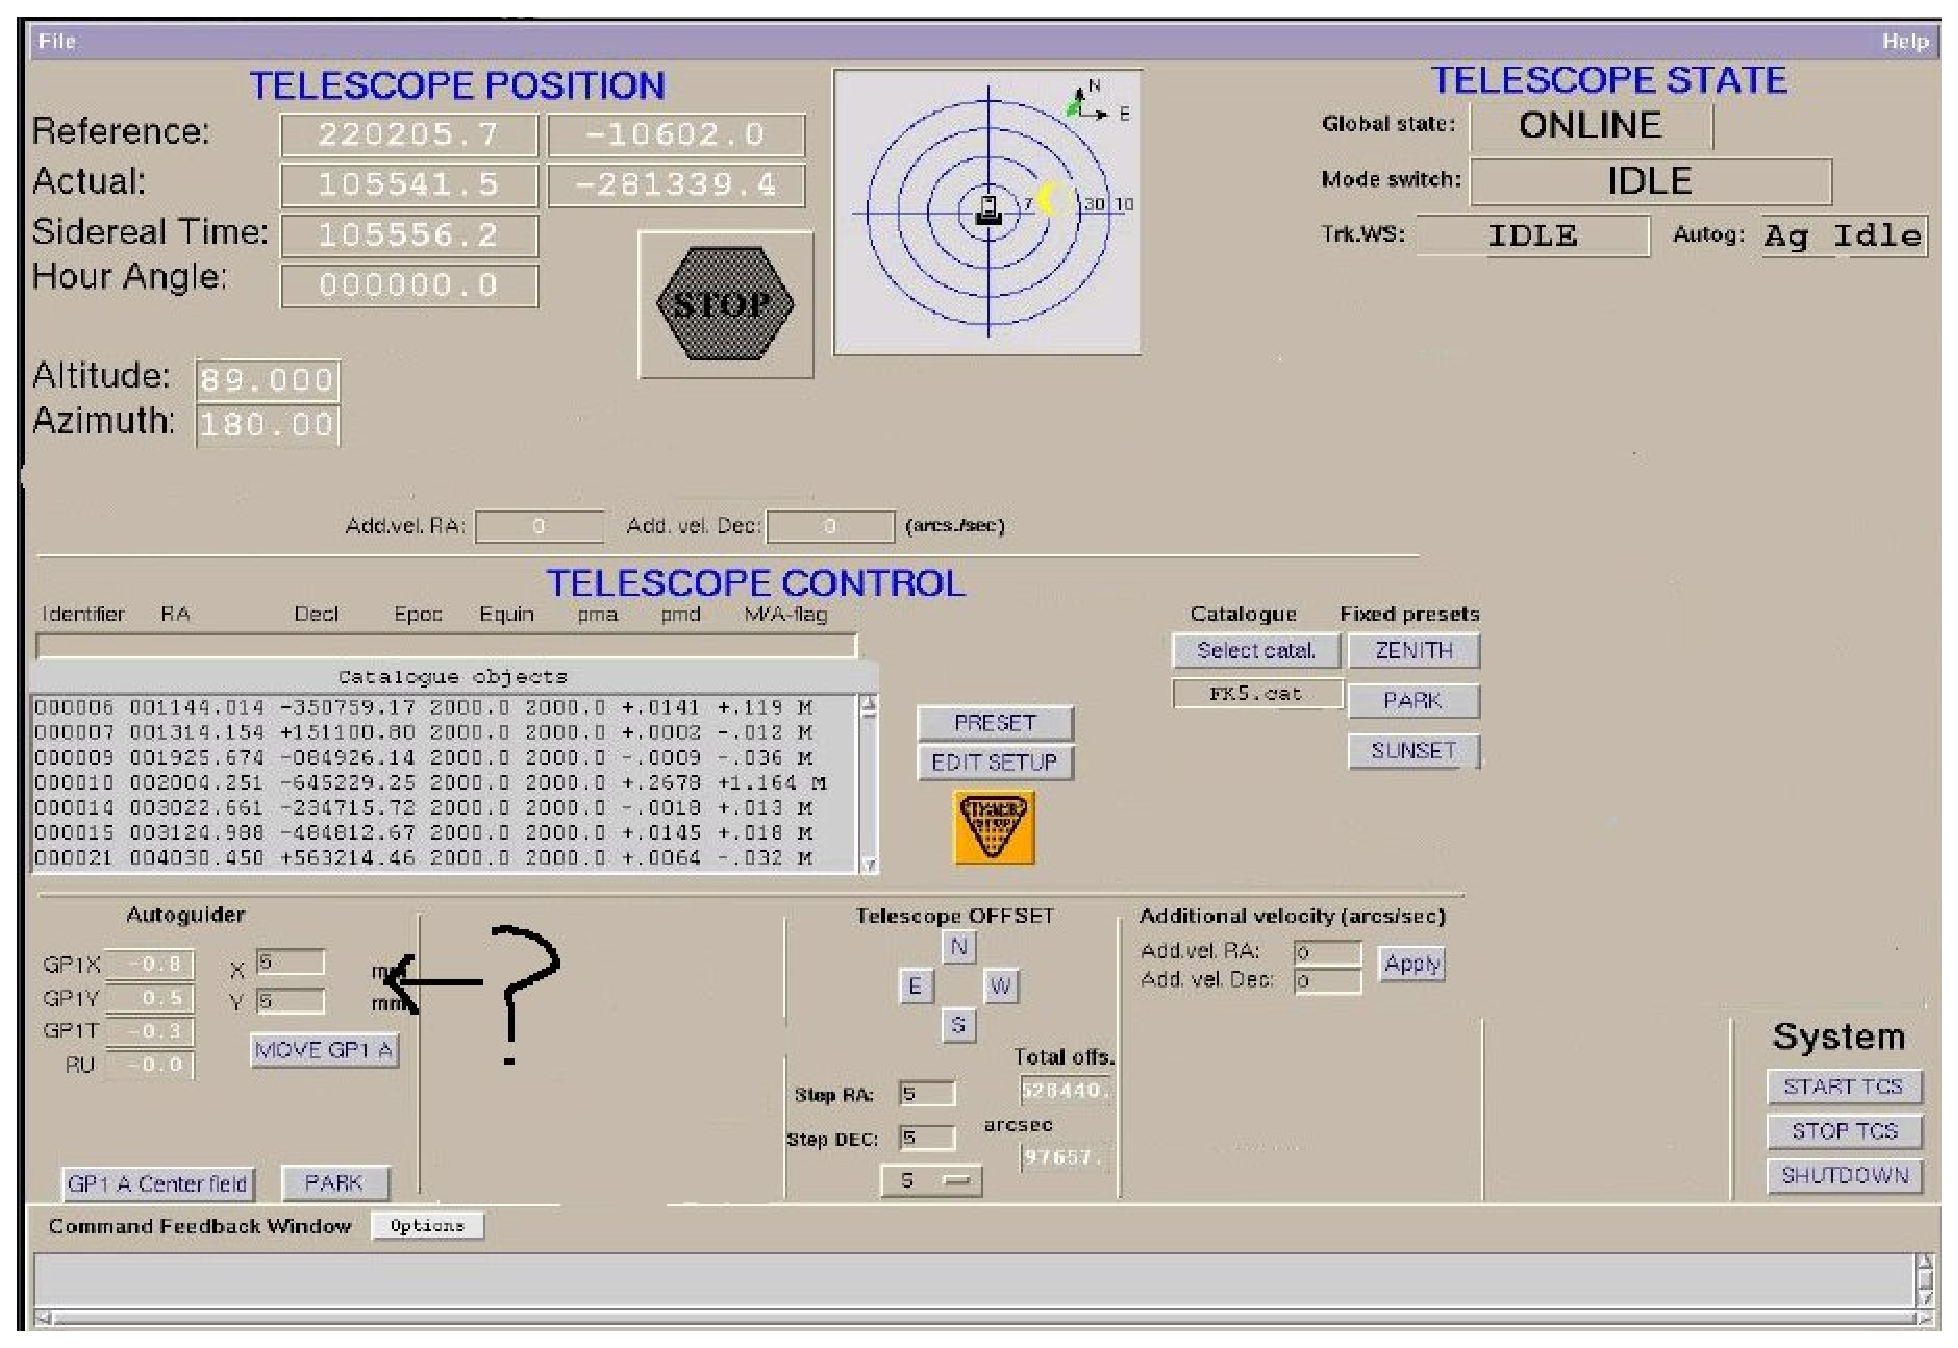
\includegraphics[scale=0.5]{tele.eps}
 \caption{Interfaz de un telescopio}
 %\label{fig:yeti}
\end{figure}

Podemos observar la confusi\'on que puede lograr y lo poco amigable que son estas 
interfaces actualmente y, en en la mayoria de los casos, tienen la informaci\'on 
necesaria para un astr\'onomo pero de forma desordenada y poco est\'andar.
 Como la mayor\'ia del tiempo el astr\'onomo est\'a en busca de nuevos descubrimientos 
que ayuden al entendimiento del universo, no se centran mucho en observar estrellas 
ya existentes, m\'as que para referencias para observar algo que podr\'ia estar 
cerca de ellas y, para ello, deben consultar cat\'alogos de estrellas, siendo un 
retraso la b\'usqueda de ella en el tiempo de observaci\'on.

\subsubsection{Identificaci\'on de problemas y deficiencias}
\textbf{Unicidad de Software:} En la actualidad existen diversos tipos de telescopios, 
los cuales est\'an implementados de manera diferente dependiendo de su dise\~nador o 
de d\'onde fueron creados. Junto con esto, aparece el problema de que cada telescopio 
posee una aplicaci\'on diferente para su control, lo que obliga a los astr\'onomos, 
operadores de telescopios y aficionados a utilizar gran parte de su tiempo aprendiendo 
a ocupar los distintos softwares para cada uno de los equipos con los que van a trabajar.

\textbf{Control:} Actualmente el control de los telescopios se debe hacer de forma local, 
es decir, los operadores de telescopios y astr\'onomos deben estar en el observatorio 
para realizar sus investigaciones, pudiendo hacerse \'este de forma remota, mejorando 
la situaci\'on para los astr\'onomos, especialmente para los que se encuentran lejos 
de los sitios de observaci\'on.

\textbf{Dificultad de Uso:} Muchos de los programas utilizados actualmente para control 
de telescopios son bastante complicados de usar, obligando a gastar una considerable 
cantidad de tiempo aprendiendo a usarlos y, tambi\'en, a usarlos frecuentemente para no 
olvidar c\'omo es que se hace.

\textbf{Seguridad del telescopio:} Es importante que el telescopio tenga medios para 
protegerse de los distintos eventos que puedan ocurrir: luminosidad alta, clima inadecuado, 
entre otros. 

\newpage

\subsection{Caracterizaci\'on del cambio}
\subsubsection{Caracter\'icticas y Potencialidades deseadas}


\paragraph{Caracter\'isticas espec\'ificas deseadas para el producto.}

	\begin{itemize}
	\item \textbf{Control por internet de telescopios:} Se quiere que el sistema 
pueda funcionar situado en cualquier parte del mundo permitiendo controlar alg\'un 
telescopio que se encuentre en otro lugar geogr\'afico.

	\item \textbf{Interfaz Gr\'afica:} El software de control de telescopios debe 
tener una interfaz agradable a los usuarios y permitir el acceso eficiente a las 
funcionalidades que se requieran, adem\'as, debe mostrar siempre en pantalla la 
informaci\'on de mayor importancia.

	\item \textbf{Reproducci\'on de lo que ve la c\'amara:} El sistema debe 
mostrar a donde apunta el telescopio en todo momento de observaci\'on, por medio de 
la c\'amara CCD.

	\item \textbf{Interacci\'on con ACS:} Es necesario que el sistema interact\'ue con 
los telescopios por medio de ACS, de manera que \'este sea el que se conecte 
directamente con los observatorios y telescopios.

	\item \textbf{Ajustar posici\'on del telescopio bajo sistema de coordenadas 
ecuatoriales:} El sistema debe poder recibir las coordenadas que se quiere observar 
y convertirlas a las coordenadas que utiliza el telescopio para poder moverlo a esa 
direcci\'on.

	\item \textbf{Mover el telescopio a la hora sideral:} El sistema debe tener la 
funcionalidad de seguir la posici\'on que se est\'a observando, ya que si no se 
hace, parecer\'ia que lo observado se ve desplazando.

	\item \textbf{Impedir observaciones a lugares con luminosidad lunar:} El sistema 
debe evitar que el telescopio apunte a direcciones con notoria luminosidad lunar, 
debido a que esta luminosidad puede da\~nar severamente los lentes del telescopio.

	\item \textbf{Mostrar modelo visual del telescopio:} Debido a que el telescopio se 
quiere manipular de forma remota, es necesario otorgar alguna forma que permita 
ver a la persona que lo est\'e operando, en qu\'e estado se encuentra. Para esto, 
el sistema debe tener un modelo visual que se comporte de la misma forma que lo 
hace el telescopio real.

	\item \textbf{Ajuste manual del telescopio:} El sistema debe permitir controlar el 
telescopio manualmente para permitir ajustes menores, que ayuden a corregir errores 
en la direcci\'on que se observa, que pudieran ocurrir por factores externos, como 
es la deflexi\'on por el peso propio del telescopio en algunas posiciones.

	\item \textbf{Detener de forma inmediata el telescopio en caso de emergencia:} El 
sistema tiene que tener una opci\'on de emergencia para detener el telescopio de 
forma inmediata para evitar cualquier da\~no que se crea que pueda ocurrir. Por 
ejemplo, da\~no por alguna variaci\'on en las condiciones clim\'aticas.

	\item \textbf{Controlar acceso a la aplicaci\'on (Sesiones):} El sistema debe tener 
acceso para los distintos usuarios, de manera que cada uno tenga su propia 
estad\'istica de lo observado.

	\item \textbf{Guardar coordenadas de observaci\'on realizadas:} El sistema debe 
guardar registro de las coordenadas observadas por cada usuario del sistema. De 
esta forma ayuda a que se puedan repetir observaciones y a realizar estudios sobre 
\'estas.

	\end{itemize}


\newpage

\paragraph{Relaci\'on de las caracter\'isticas con los problemas identificados.}

	\begin{itemize}

	\item El control por internet va a ayudar a solucionar el problema de tener 
que estar en el lugar de observaci\'on al momento de controlar al telescopio.

	\item La interfaz gr\'afica va a ayudar a disminuir la dificultad de uso, 
ocultando informaci\'on que no sea requerida en todo momento, pero permitiendo 
verla de manera sencilla e intuitiva.

	\item La reproducci\'on de lo que est\'a viendo el telescopio es de gran 
utilidad para la experiencia remota, debido a que sino hiciera esto, no se podr\'ia 
ver lo que est\'a viendo el telescopio, hasta que se enviara alg\'un informe a 
quien controlaba el telescopio.

	\item La interacci\'on con ACS es una de las caracter\'isticas principales 
para el control gen\'erico de telescopios y el control de telescopios por medio 
de internet, pues es esta plataforma la que permite la comunicaci\'on con los 
telescopios en los diferentes observatorios del mundo.

	\item Mover el telescopio a la hora sideral reduce la dificultad de uso 
para el seguimiento de la observaci\'on de alg\'un objeto, puesto que nos permite 
ver en todo momento al objeto deseado, sin necesidad de realizar tareas adicionales.

	\item Al impedir que el telescopio apunte a lugares con luminosidad lunar 
se reduce la dificultad de uso, puesto que no es necesario estar preguntandose 
todo el tiempo si el telescopio va a apuntar a lugares potencialmente da\~ninos 
para el mismo. Adem\'as, aumenta la seguridad del telescopio puesto que lo proteje 
de la luz lunar, uno de los factores m\'as comunes que da\~nan al telescopio.

	\item El modelo visual soluciona un aspecto muy importante de la dificultad 
de uso para el control a trav\'es de internet, ya que con este se puede saber en 
todo momento hacia d\'onde est\'a apuntando f\'isicamente el telescopio, d\'andonos 
un apoyo gr\'afico de lo que estamos haciendo. De la misma forma, tambi\'en ayuda 
a los que operan el telescopio de forma local, aunqiue ellos podr\'ian verlo 
directamente, puede ser m\'as c\'omodo verlo en la misma pantalla que est\'an trabajando.

	\item El ajuste manual ayuda a disminuir la dificultad de uso del sistema, 
puesto que con este, no es necesario intuir una direcci\'on parecida a la que 
estamos observando de manera que se vea lo que debiera, sino que simplemente 
lo movemos manualmente hasta donde debiera estar.

	\item Al dar la posibilidad de detener manualmente al telescopio, aumentamos 
en gran medida su seguridad, puesto que mediante esta opci\'on, podemos protegerlo 
de factores que no esperabamos, como son las variaciones inesperadas en el clima. 

	\item El guardar coordenadas de observaci\'on realizadas por sesi\'on facilita 
la dificultad de uso del sistema, ya que para gente no muy experimentada en el tema, 
permite repetir las observaciones hechas otros d\'ias.

	\end{itemize}

\subsubsection{Restricciones}

\begin{itemize}

\item \textbf{Econ\'omicas:} El software no presenta restricciones econ\'omicas, 
puesto que tanto el sistema operativo, como las herramientas de desarrollo que se 
van a utilizar, son gratuitas. Por otro lado, los componentes de hardware como son 
el telescopio para pruebas y la c\'amara CCD si tienen un costo, pero en este caso 
ser\'an facilitados por el cliente. Es por esto, que no vemos restricciones 
econ\'omicas peligrosas.

\item \textbf{Sociales y Culturales:} Los usuarios actuales de los programas que 
controlan telescopios han tenido que usar diferentes aplicaciones para distintos 
telescopios a lo largo del tiempo que han dedicado a esto, prefiriendo quiz\'as, 
el que usan actualmente, ya sea por costumbre o por gusto personal. Esto puede 
dificultar que se acostumbren a usar el sistema propuesto, pero se espera que el 
sistema final sea intuitivo y amigable, de manera que esto no debiera suceder.

\item \textbf{Tecnol\'ogicas:} En el aspecto tecnol\'ogico es importante destacar 
que las pruebas iniciales no necesariamente se har\'an con un telescopio de 
observatorio, en estos casos se utilizar\'a para las pruebas telescopios para 
aficionados, puesto que los costos de observaci\'on son elevados.

%%%%\item \textbf{Institucionales:}


\end{itemize}

\subsection{An\'alisis de las alternativas de soluci\'on}
\subsubsection{Alternativa 1: Desarrollo de Software basado en ACS} %%%% TOMAS
Desarrollo de un producto de software basado en la plataforma ACS que sea gen\'erico,
es decir, que nos permita controlar cualquier telescopio por medio del mismo
programa, sin la necesidad de tener un programa diferente para cada telescopio.

Se utiliza un computador como estaci\'on de trabajo de quien opere el telescopio, 
en donde todo el control se realizar\'a por medio de una interfaz gr\'afica. Este
computador requerir\'a tener acceso a internet para poder obtener componentes desde
ACS y para comunicarse con el telescopio que se quiera controlar.

La interfaz gr\'afica mostrar\'a a quien opere el telescopio el estado actual del
mismo, pudiendo verse lo que est\'a observando el telescopio por medio de la
c\'amara CCD y la disposici\'on f\'isica en que se encuentra el telescopio, por medio
del modelo hecho en OpenGL del mismo.

Es importante notar que al utilizar la plataforma ACS para la distribuci\'on de 
componentes de software, se podr\'ian usar componentes realizados por otras personas, 
asi como realizar cambios en componentes que utiliza nuestro software, obteniendo un
producto de alta modularidad, enfocado al trabajo por componentes.

\subsubsection{Alternativa 2: Reutilizaci\'on de software de control de telescopios} %%%% TODOS
Realizar un programa que reutilice las aplicaciones existentes detectando el telescopio
que se quiere controlar y luego llamando a la aplicaci\'on correspondiente.

En m\'as detalle, consiste en realizar una base de datos que contedr\'ia una 
asociaci\'on entre los telescopios y el programa que los controla. Para reducir
el tama\~no de las distribuciones se utilizar\'ia un sistema distribuido de los
distintos programas, de manera que cuando se detecte el telescopio que se quiera
controlar, se haga una petici\'on de descarga el software requerido para su control.

En esta soluci\'on aparecen muchos problemas, destacando los problemas legales en 
cuanto a tema de patentes y derechos de autor, los problemas de diferencia de 
interfaz gr\'afica, recursos necesarios del equipo poco claros y variables seg\'un 
el telescopio que se controle.

De los derechos legales lo principal ser\'ia el tema de las patentes y los derechos
de autor, ya que utilizar\'iamos programas hechos por otras personas que muchas 
veces tienen patentes y est\'a restringido su uso por decisi\'on de sus autores. 
Por la gran cantidad de programas existentes, nos ser\'ia imposible hacer peticiones 
a cada uno para usar su programa.

Debido a que en esta soluci\'on llamamos a programas hechos por otras personas, para
cada telescopio tendr\'iamos una interfaz gr\'afica diferente, lo cual deja uno de 
los principales problemas sin mejorar.

Ya que se utilizan distintos programas dependiendo del telescopio que se quiera 
controlar, no podr\'ia asegurarse los requerimientos del equipo para el control del
telescopio. Se podr\'ia poner el mayor de los casos, pero no es lo m\'as adecuado.

\subsection{Soluci\'on recomendada} %%%% TOMAS
La mejor soluci\'on que encontramos es la alternativa 1, en la cual se piensa construir
un producto de software gen\'erico basado en ACS, el cual se acopla bastante bien 
con los requerimientos del cliente.

Este producto deber\'a ser modular basado en componentes con el estilo que ACS nos
impone, por lo que se tendr\'an algunos componentes sobre esta plataforma, mientras que
otros ir\'an junto con el software principal. Es importante hacer la separaci\'on
de las capas de comunicaci\'on, interfaz gr\'afica y software, para simplificar la
mantenci\'on del producto al tener las funcionalidades separadas.

Se eligi\'o esta alternativa, porque en la actualidad no hay productos que controlen
telescopios de forma gen\'erica, y esto es algo muy importante para enfocar los esfuerzos
de observaci\'on en las observaciones mismas y no en aprender a utilizar los programas
asociados al control de telescopios.


\newpage
\section{T\'ecnicas y Herramientas de desarrollo} %%% CARLOS
\subsection{Modelo de desarrollo}
Las caracter\'isticas m\'as importantes del proyecto Hevelius con
respecto a la elecci\'on de un modelo de desarrollo se expone en lo
siguiente. Primero se consideran las propiedades del producto:

\begin{itemize}
\item \textbf{Complejidad del Proyecto:} una estimaci\'on informal del proyecto
  muestra una complejidad media, la cual permite la finalizaci\'on del
  proyecto dentro del plazo predeterminado;
\item \textbf{Solidez de los Requerimientos:} c\'omo el producto a
  desarrollar est\'a inserto en un proyecto de investigaci\'on, es posible que
  los requerimientos capturados durante el an\'alisis sean completos en su generalidad,
  sujetos a pocos cambios.
\item \textbf{Innovaci\'on del Producto:} en vista de que la principal caracter\'istica
  del proyecto es la b\'usqueda de la generalidad en el control de telescopios, existen 
  errores que durante el desarrollo se descubrir\'an, lo que nesecitar\'a cambios en el
  c\'odigo implementados o en el dise\~no del software.
\end{itemize}

Adem\'as, el ambiente del desarrollo tiene las siguientes caracter\'isticas:

\begin{itemize}
\item \textbf{Tama\~no del Equipo:} cuatro personas durante la planificaci\'on y el 
  desarrollo del proyecto.
\item \textbf{Recursos Disponibles:} nuestro cliente nos provee de un lugar f\'isico, 
  computadores y un telescopio para el desarrollo de nuestro proyecto.
\item \textbf{Tratamiento de los miembros del equipo entre s\'i:} informal, ya
  que existen lazos de amistad anteriores a la formaci\'on del grupo de trabajo.
\item \textbf{Proyecci\'on en el tiempo:} se cuenta con un plazo determinado,
  debido a que el proyecto pretende ser parte de la Feria de Software 2007, 
  de aproximadamente cinco meses a partir de la fecha de entrega de este informe.
\end{itemize}


Teniendo en cuenta el conjunto de caracter\'isticas del proyecto, se
decide usar un modelo de desarrollo en fases para la
mayor\'ia de las tareas; espec\'ificamente se prevee el uso del \emph{Modelo
Iterativo} en el trabajo. Sin embargo, no podemos desechar el \emph{Modelo
Incremental}, debido a la posible implementaci\'on de m\'odulos no considerados en un
principio en el software.

Habiendo elegido este m\'etodo de desarrollo, es necesario realizar las
siguientes actividades durante el desarrollo para el modelo iterativo:

\begin{enumerate}
\item \textbf{Pruebas:} los requerimientos (funcionales o no-funcionales) deben
  ser transformados en pruebas automatizables.
\item \textbf{Construir:} el c\'odigo producido debe estar siempre en un
  estado que permite su compilaci\'on.
\item \textbf{Escuchar:} La comunicaci\'on a lo largo del desarrollo del proyecto
con el cliente, debe ser fluida, esto para atender a las 
  verdaderas necesidades y para solicitar sus comentarios sobre el
  estado del desarrollo, y posibles cambios en los requerimientos.
\item \textbf{Dise\~nar:} para facilitar el proceso de codificaci\'on y permitir el
  trabajo paralelo de grupos independientes, hay que contar con un
  dise\~no del sistema.
  Esta actividad hay que hacerla durante todo el tiempo del desarrollo,
  adapt\'andose a funcionalidad agregada.
\item \textbf{Comunicaci\'on dentro del equipo:} es importante
  que la comunicaci\'on entre los integrantes funcione
  muy bien, es decir, todos deben saber la mayor\'ia del tiempo en qu\'e
  est\'an trabajando los dem\'as y cu\'ales son los cambios realizados por
  ellos.
\end{enumerate}

Para el componente planificado, hay que hacer un plan inicial de
recursos y tiempo necesitado, para lo que sirve este documento, y
controlar el progreso actual del proyecto, para lo que sirven los
\emph{fichas de estado}.

Adem\'as es necesario documentar el dise\~no actual del programa.


\subsection{Herramientas y t\'ecnicas de soporte para el desarrollo}
\subsubsection{T\'ecnicas a utilizar en el desarrollo del proyecto}

Durante el desarrollo del proyecto se utilizar\'a el m\'etodo de desarrollo en fases iterativo, 
ya que como hay ejecutables desde el mismo comienzo del proyecto, nuestro cliente puede examinarlos 
y proponer los cambios necesario (si los hubiera). Tambi\'en la empresa tiene una r\'apida 
retroalimentaci\'on de lo que funciona y lo que no, ya que las pruebas se realizan desde el 
comienzo mismo del proyecto y no se debe esperar al final para hacer las modificaciones necesarias.\\

Se opt\'o por este m\'etodo debido a la seguridad que da su planificaci\'on al cliente, ya que \'el 
puede \textit{ver} en que se est\'a trabajando y cuales ser\'an los pr\'oximos pasos a seguir.\\

Dentro de los lenguajes de programaci\'on, nuestro cliente nos requiri\'o el uso de ciertos lenguajes 
de programaci\'on, debido a est\'andares interncionales. Estos lenguajes son: C, C++, Java y Phyton. 
Todos los integrantes del grupo, cuentan con conocimientos en C, Java y otros en C++.\\

Es posible que se utilice alguna herramienta de dise\~no vectorial para la creaci\'on de las gr\'aficas 
a utilizar en el software, pero a\'un no se ha descartado ni confirmado ninguna de ellas.\\


\subsubsection{Herramientas o plataformas espec\'ificas a utilizar}

La plataforma operacional de Hevelius est\'a constituida por el Sistema Operativo Linux Fedora Core, 
debido a que es esta la distribuci\'on utilizada por nuestro cliente para desarrollar software. Esta 
distribuci\'on a su vez debe contar con el framework ACS en su versi\'on 6.0 o superior.\\


\subsection{Personal y capacitaci\'on del grupo de desarrollo}
\begin{itemize}

    \item Personal del equipo del proyecto.
		
La empresa DevNull cuenta actualmente con cuatro miembros, de los cuales se har\'a una breve descripci\'on de sus perfiles personales, paso primordial para conocer al equipo de trabajo:

	\begin{description}
		
	\item[Marina Alejandra Pilar Daza].

Alumna de cuarto a\~no de ingenier\'ia civil inform\'atica de la UTFSM, se caracteriza 
por ser una persona responsable y comprometida con los trabajos asignados. Tiene 
capacidad de liderazgo, a pesar que no siente mucha motivaci\'on por utilizarlo. 

Adem\'as, podemos rescatar su manera directa de decir las cosas, que hacen que 
exista una buena relaci\'on en el equipo de trabajo y, no existan malas interpretaciones 
de las cosas y el buen trabajo en equipo que realiza.

Dentro de sus areas de inter\'es, se encuentra la inform\'atica, la historia universal 
y lectura de cualquier tipo de libros; a pesar que a\'un no tiene un \'area especifica 
a la cual se va a dedicar, actualmente se centra en la \'area de Sistemas Computacionales, 
lo cual se puede aprecia al ver que trabaja en el laboratorio de Computaci\'on en el 
departamento de inform\'atica de la UTFSM, del cual ha adquirido experiencia tanto en 
el \'ambito t\'ecnico como en el humano, al tener contacto con otras personas, ya 
sean con usuarios o el mismo trabajo en equipo que se tiene que llevar en un trabajo como ese.


                \begin{itemize}
                \item{Conocimientos T\'ecnicos:}
                        \begin{itemize}
                        \item{Administrador de Sistemas:}  Cuentas, Bases de Datos.
                        \item{Sistemas Operativos:} Microsoft Windows, Linux.
                        \item{Lenguajes de Programaci\'on:} C, C++, Basic, Visual Basic, Java, PHP, ASP, Javascript, Scheme, Prolog, Bash, Perl.
                        %\item{Librer\'ias:} SDL, GTK, QT, CUPS, STL.
                        \end{itemize}
                \end{itemize}



	\item[Tom\'as Ignacio Staig Fern\'andez].

Persona met\'odica y anal\'itica. Es una persona que se esfuerza por lograr que
las cosas funcionen bien, para lo cual utiliza tanto los conocimientos que ha
obtenido como soluciones que el mismo pueda ingeniar.

Muestra inter\'es principalmente por las \'areas de Modelos y M\'etodos
cuantitativos y por la de Sistemas Computacionales. Esto no quita que
le guste desarrollar software, sino que remarca el hecho de que le gusta
desarrollar para solucionar problemas.

Posee un buen uso del lenguaje espa\~nol oral y escrito, pero destaca por tener
buen manejo del idioma ingl\'es, tanto oral como escrito, estando certificado
por la evaluaci\'on First Certificate in English de la Universidad de Cambridge.

Sus hobbies son el volleyball, tenis y juegos de computador. Dentro de \'estos
destaca que se encuentra en la rama de Volleyball de la Universidad T\'ecnica
Federico Santa Mar\'ia.

\begin{itemize}
        \item{Conocimientos T\'ecnicos:}
        \begin{itemize}
                \item{Sistemas Operativos:} Microsoft Windows, Linux.
                \item{Lenguajes de Programaci\'on:} C, C++, Visual Basic, Java, PHP, ASP, Javascript, Scheme, Prolog, Bash, Perl, HTML.
                \item{Librer\'ias:} OpenGL.
        \end{itemize}
\end{itemize}




	\item[Esteban Ignacio Espinoza Mart\'inez].
Estudiante de cuarto a\~no de Ingenier\'ia Civil Inform\'atica de la UTFSM.
Su capacidad de integraci\'on le permite desenvolverse de buena manera en 
equipos de trabajo. Su capacidad de superaci\'on y esfuerzo le permiten 
cumplir siempre con todas las metas que se propone.

Se inclina hacia el \'area de Sistemas Computacionales y Programaci\'on, 
esta ultima vista en los trabajos como ayudante de Laboratorio de Programaci\'on de la UTFSM en diversos lenguajes.
Posee dominio del idioma Ingl\'es a nivel b\'asico (oral) e intermedio (t\'ecnico y escrito).
Sus hobbies son tocar clarinete, o\'ir Jazz y videojuegos.


                \begin{itemize}
                \item{Conocimientos T\'ecnicos:}
                        \begin{itemize}
                        \item{Sistemas Operativos:} Microsoft Windows, Linux.
                        \item{Lenguajes de Programaci\'on:} C, Visual Basic, Java, PHP, ASP, Javascript, Scheme, Prolog, Perl.
                        \end{itemize}
                \end{itemize}




	\item[Carlos Alberto Guajardo Miranda].

Alumno responsable, con alto grado de compromiso en sus labores cotidianas. 
Posee gran capacidad de liderazgo y organizaci\'on, lo cual complementado con 
sus conocimientos t\'ecnicos lo hacen cumplir la mayor\'ia de sus metas propuestas.

Sus intereses van por el \'area de Sistemas Computacionales y la Programaci\'on. 
Esto se demuestra con el trabajo que realiza en la Unidad de Servicios de Computaci\'on 
e Internet del Departamento de Inform\'atica de la UTFSM.

Posee dominio del idioma Ingl\'es a nivel b\'asico (t\'ecnico y escrito).
Se destaca sus conocimientos e inter\'es en diferentes deportes (f\'utbol, tenis, basketball, etc.).

Sus hobbies son el f\'utbol y videojuegos.

                \begin{itemize}
                \item{Conocimientos T\'ecnicos:}
                        \begin{itemize}
                        \item{Administrador de Sistemas:} Web, SVN, Bases de Datos.
                        \item{Sistemas Operativos:} Microsoft Windows, Linux.
                        \item{Lenguajes de Programaci\'on:} Pascal, C, C++, Visual Basic, Java, HTML, PHP, ASP, Javascript, Prolog, Bash, Perl.
                        %\item{Librer\'ias:} SDL, GTK, QT, CUPS, STL.
                        \end{itemize}
                \end{itemize}




	\end{description}


	\item Perfil del equipo ideal para el proyecto.

Para la empresa DevNull, el equipo ideal requerido para este proyecto requiere que cumpla con las siguientes caracter\'isticas:

		\begin{itemize}

		\item{Conocimientos de Astronom\'ia:} Esencial es el conocimiento sobre las coordenadas 
astron\'omicas que se usan en la actualidad, tanto su aplicaci\'on en la observaci\'on como la transformaci\'n 
a otras coordenadas.
		\item{Conocimientos sobre Telescopios:} Se requiere conocer como son los diferentes tipos 
de movimientos que poseen los telescopios, el por qu\'e de ese movimiento y las coordenadas que m\'as 
``le acomoda''.
		\item{Conocimientos de Lenguajes de Programaci\'on:} 
			\begin{itemize}
			%%%% C++, JAVA, C , LATEX, PHYTON
			\item{Java:} En este lenguaje de programaci\'on orientado a objetos se basar\'a 
la interfaz de nuestro software.
			\item{C, C++, Phyton:} Estos lenguajes de programaci\'on ser\'an usados en la creaci\'on 
de modulos y componentes del software.
			\item{\LaTeX:} Este lenguaje ser\'a usado para generar la documentaci\'on que 
surge a trav\'es de los entregables o a partir de la propia investigaci\'on que surge durante el avance 
del trabajo.
			\end{itemize}
		\item{Conocimientos de Software:} Es esencial, en el desarrollo de Hevelius, que se tenga 
conocimiento del framework ACS en su versi\'on 6.0 o superior, debido a que en este framework se desarrolla 
el proyecto.
		\item{Conocimientos de Sistemas Operativos:} Se requiere un conocimiento en espec\'ifico del 
sistema operativo Fedora, el cual se encuentra actualmente en la version 6, debido a que es el sistema sobre 
el cual funciona ACS. 

		\end{itemize}

A partir de los datos tabulados, se puede decir que la mayor\'ia de los recursos t\'ecnicos requeridos por el equipo son cubiertos. 

        %\end{itemize}

        \item An\'alisis de insuficiencias de los miembros del equipo, si las hubiere.

A partir de lo anterior, las insufiencias que se deber\'ian cubrir son los siguientes:

		\begin{itemize}
		\item{Falta de capacitaci\'on en Astronom\'ia y ACS:} En conjunto los 
miembros del equipo s\'olo mantienen nociones b\'asicas de astronom\'ia, por lo que 
limita el trabajo por el poco entendimiento t\'ecnico que se posee, lo que tambi\'en 
trae problemas de comunicaci\'on con el cliente.
		\end{itemize}

        \item Programa de mejoramiento (capacitaci\'on, mentor\'ia, incorporaci\'on 
de nuevos miembros...), indicando espec\'ificamente acciones a realizar y plazos.

Para el mejoramiento de las insuficiencias detectadas, el equipo recurrir\'a al 
siguiente plan de accion:

		\begin{itemize}
		\item{Falta de capacitaci\'on en Astronom\'ia y ACS:} Para mejorar esta 
insuficiencia, nuestro cliente nos realizar\'a workshops tanto de astronom\'ia como de ACS, 
con el fin de interiorizarnos en estos temas y as\'i poseer todos el mismo grado de conocimiento.
		\end{itemize}

\end{itemize}



\newpage
\section{Gesti\'on de Riesgos} %%% ESTEBAN
\subsection{An\'alisis de riesgos}
\begin{itemize}
\item{\bf{Riesgos de Negocio:}} 
\begin{itemize}
\item{\bf{Poca escalabilidad de Hevelius con respecto a telescopios profesionales.}}

Un gran riesgo es que una vez terminado el proyecto, al intentar ser probado en un telescopio profesional, no sea lo suficientemente escalable y termine por no realizar un funcionamiento adecuado.
\end{itemize}

\item{\bf{Riesgos del Proyecto:}}
\begin{itemize}
\item{\bf{Ausencia de alg\'un integrante del proyecto}}

La ausencia de alg\'un integrante del equipo de trabajo implicar\'ia un  mayos esfuerzo por parte del resto del equipo a dem\'as de incrementar el tiempo de desarrollo del proyecto, lo cual podr\'ia traer serios problemas.

\item{\bf{Incumplimiento con fechas.}}

Todos los proyectos tienen una fecha limite para cada etapa y sus respectivas entregas. Un riesgo importante es el incumplimiento de las fechas finales, las cuales corresponden a la presentaci\'on del proyecto en La Feria de Software.	

\item{\bf{Telescopio Amateur no disponible}}

Para la presentaci\'on de la feria, Hevelius ser\'a probado en un telescopio amateur el cual es propiedad de ACS-UTFSM Group, por lo que la disponibilidad de este se puede ver afectada para dicha presentaci\'on.

\item{\bf{Estimaci\'on del proyecto err\'onea}}

Una mala estimaci\'on del proyecto, en cuanto a complejidad y desarrollo implicar\'ia un gran riesgo, puesto que podr\'ia darse el caso en que no se logre finalizar el proyecto dentro de la fecha estimada.

\item{\bf{Falta de conocimiento en cuanto al \'area de desarrollo}}

Hevelius al tratarse de un proyecto que esta en el \'area de la astronom\'ia, obliga necesariamente al equipo de trabajo familiarizarse con t\'erminos e informaci\'on propia de dicha \'area, lo cual implica una capacitaci\'on para el equipo de manera de poder visualizar de mejor manera el problema y poder desarrollar una mejor soluci\'on, a dem\'as de permitir una mejor obtenci\'on de informaci\'on de parte del cliente. 

\item{\bf{No cumplimiento con los est\'andares del proyecto ALMA-CONICYT}}

Hevelius al formar parte del proyecto ALMA-CONICYT debe cumplir ciertos est\'andares, por lo que alg\'un tipo de incumplimiento producir\'ia conflictos en cuanto a utilizaci\'on y una mala evaluaci\'on del proyecto por parte de nuestro cliente.

\end{itemize}


\item{\bf{Riesgos T\'ecnicos:}}
\begin{itemize}
\item{\bf{Mala elecci\'on en cuanto a lenguajes de programaci\'on.}}

Una mala elecci\'on del lenguaje de programaci\'on implicar\'ia un gran riesgo, puesto que producir\.ia un mayor esfuerzo en la creaci\'on de funciones propias del proyecto, lo cual puede retrasar el desarrollo de manera exponencial si no se hace adecuadamente.

\item{\bf{Compleja interfaz gr\'afica para el usuario.}}

Hevelius entre otros objetivos busca ser una herramienta amistosa para los operadores de telescopio, por lo tanto el tener una interfaz muy engorrosa volver\'ia la utilizaci\'on del proyecto muy compleja y poco entendible, para esto se deben utilizar herramientas y t\'ecnicas que permitan un desarrollo de interfaz amigable.

\item{\bf{Pocas pruebas realizadas al proyecto.}}

Una herramienta importante en el desarrollo de software es la fase de pruebas, una vaga fase de pruebas al proyecto puede significar errores que no son identificados en la etapa correcta y que conlleva a errores en futuras etapas lo que implica un cambio en la estructura del proyecto, los cuales son mas costosos a medida de que el proyecto avanza.
\end{itemize}
\end{itemize}
\begin{tabular}{||l | c | r||}
\hline
\textbf{Nombre del Riesgo} & \textbf{Ocurrencia} & \textbf{Impacto} \\ 
\hline
Poca escalabilidad de Hevelius con respecto a telescopios profesionales. & Muy Alto & Muy Alto\\
\hline
Ausencia de alg\'un integrante del proyecto & Baja & Muy Alto\\
\hline
Incumplimiento con fechas & Media & Alto\\
\hline
Telescopio amateur no disponible & Baja & Muy Alto\\
\hline
Estimaci\'on err\'onea del proyecto & Media & Muy Alto\\
\hline
Falta de conocimiento en cuanto al \'area de desarrollo & Media & Alto\\
\hline
No cumplimiento con los est\'andares del proyecto ALMA-CONICYT & Baja & Alto\\
\hline
Mala elecci\'on en cuanto a lenguajes de programaci\'on & Baja & Alto\\
\hline
Compleja interfaz grafica para el usuario & Alta & Muy Alto\\
\hline
Pocas pruebas realizadas al proyecto & Media & Alto\\
\hline
\end{tabular}

Para priorizar los riesgos es necesario evaluar tanto su ocurrencia como el impacto que provocar\'ia en el proyecto.
Se debe crear un consenso en el equipo de trabajo para poder tomar la decisi\'on correcta.

\begin{enumerate}
	\item Poca escalabilidad de Hevelius con respecto a telescopios profesionales.
	\item Compleja interfaz grafica para el usuario.
	\item Estimaci\'on del proyecto err\'onea.
	\item Falta de conocimiento en cuanto al \'area de desarrollo.
	\item Pocas pruebas realizadas al proyecto.
	\item No cumplimiento con las fechas.
	\item Mala elecci\'on en cuanto a lenguajes de programaci\'on.
	\item Telescopio amateur no disponible.
	\item Ausencia de alg\'un integrante del proyecto.
	\item No cumplimiento con los est\'andares del proyecto ALMA-CONICYT.
\end{enumerate}

\newpage
\subsection{Preparaci\'on para control de riesgos}

\begin{table}[h!]
\centering
\begin{tabular}{|p{35mm}|p{35mm}|p{35mm}|p{35mm}|}
\hline
ID 1 & \multicolumn{3}{|p{105mm}|}{Poca escalabilidad de Hevelius con respecto a telescopios profesionales.}\\ \hline
Prioridad: 1 & \multicolumn{3}{|p{105mm}|}{Clase: Riesgo de Negocio}\\ \hline
\multicolumn{2}{|p{70mm}|}{Probabilidad: Muy Alta} & \multicolumn{2}{|p{70mm}|}{Impacto: Muy Alto}\\ \hline
\multicolumn{4}{|p{148mm}|}{Descripci\'on: La capacidad del proyecto de adaptarse a los cambios a futuro y de adem\'as poder adaptarse a otros tipos de telescopios y principalmente a un telescopio profesional.}\\ \hline
\multicolumn{2}{|p{70mm}|}{Per\'iodo: Todo el proyecto} & \multicolumn{2}{|p{70mm}|}{Estado: Latente}\\ \hline
\multicolumn{4}{|p{148mm}|}{Contexto: 
La escalabilidad que se requiere en Hevelius debe ser capaz de poder conectarse principalmente a un telescopio profesional y posteriormente ser lo mas gen\'erico posible.}\\ \hline
\multicolumn{4}{|p{148mm}|}{Plan de Mitigaci\'on: 
Los primero tres artefactos a considerar para mitigar este riesgo se
Aplicar\'an en la etapa de an\'alisis, los cuales permiten bosquejar los elementos del sistema,
captar aquellos elementos sustituibles u omitibles, adem\'as se podr\'an visualizar los
futuros componentes, con esto adaptar el modelo y ver, a grandes rasgos, el modo de implementaci\'on de ellos.
Un artefacto utilizado para mitigar este riesgo en la etapa de construcci\'on, ser\'a probar el funcionamiento a 
trav\'es de prototipos funcionales de prueba, con lo
cual se generar\'a una retroalimentaci\'on y se 
podr\'a interpretar de manera mas fidedigna el sistema en construcci\'on. Por \'ultimo, se considera como alternativa 
de soluci\'on a este riesgo el car\'acter modular que presentara Hevelius a travez de los componentes de ACS, de manera que se puedan a\~nadir nuevas funcionalidades sin afectar a las ya existentes y permitir un software lo m\'as generico posible por intermedio de estos modulos. Por lo tanto, una investigaci\'on acerca de este 
tema podr\'a medir la factibilidad de uso y aplicaci\'on.}\\ \hline
\multicolumn{4}{|p{148mm}|}{Plan de contingencia: 
Replantear la modularidad del
sistema, esto significa, volver a analizar los m\'odulos para encontrar posibles subsecciones
y reformularlas. Luego de esto, a.nadir nuevos
m\'odulos que permitan adaptar nuevos componentes de hardware en el sistema, junto con la vinculaci\'on a la interfaz de usuario.}\\ \hline
\multicolumn{4}{|p{148mm}|}{Resoluci\'on:
La resoluci\'on de este riesgo consiste en asignar \'areas y tareas espec\'ificas a cada integrante del equipo de trabajo, para lograr la profundidad en los temas que se necesitan al desarrollar la soluci\'on.}\\ \hline
\end{tabular}
\caption{Hoja Control de Riesgo: ID1}
\label{table:control_riegos_1}
\end{table}

%% RIESGO 2 %%%
\newpage
\begin{table}[h!]
\centering
\begin{tabular}{|p{35mm}|p{35mm}|p{35mm}|p{35mm}|}
\hline
ID 2 & \multicolumn{3}{|p{105mm}|}{Compleja interfaz grafica para el usuario.}\\ \hline
Prioridad: 2 & \multicolumn{3}{|p{105mm}|}{Clase: Riesgo T\'ecnico}\\ \hline
\multicolumn{2}{|p{70mm}|}{Probabilidad: Alta} & \multicolumn{2}{|p{70mm}|}{Impacto: Muy Alto}\\ \hline
\multicolumn{4}{|p{148mm}|}{Descripci\'on: La complicaci\'on que puede generar la construcci\'on de cada uno de los elementos
que componen la interfaz de usuario es un factor que puede retrasar el proyecto.}\\ \hline
\multicolumn{2}{|p{70mm}|}{Per\'iodo: Todo el proyecto} & \multicolumn{2}{|p{70mm}|}{Estado: Latente}\\ \hline
\multicolumn{4}{|p{148mm}|}{Contexto:
La interfaz de usuario corresponde al nexo de interacci\'on entre el usuario y
el sistema, adem\'as en \'el se encuentran expl\'icitos la mayor\'ia de los requerimientos del
proyecto. El problema que puede generar la construcci\'on de esta interfaz, es la demora
en el desarrollo de algunos de los elementos que la componen, as\'i como la correcta
elecci\'on de las herramientas para desarrollarla. A dem\'as cabe destacar que de por si la interfaz para un proyecto como Hevelius es muy compleja, por lo que una mayor complicaci\`on significar\'ia un retraso importante.}\\ \hline
\multicolumn{4}{|p{148mm}|}{Plan de Mitigaci\'on:
Como la interfaz es lo que finalmente el usuario vera del proyecto es necesario que sea el mismo quien nos provea de la informaci\'on necesaria para el correcto desarrollo de esta. Tambi\'en es factible la investigaci\'on en manuales y t\'ecnicas de desarrollo de interfaces para tener una mayor gama de  ideas y herramientas que permitan mitigar este riesgo.}\\ \hline
\multicolumn{4}{|p{148mm}|}{Plan de contingencia:
El plan de contingencia implica la reformulaci\'on de las interfaces realizadas hasta el momento y de buscar una retroalimentaci\'on proveniente de los mismo usuarios del proyecto, as\'i como de asesoramiento por parte de profesionales o gente experimentada en el tema de desarrollo de interfaces graficas.
Tambi\'en es factible el dedicar una mayor cantidad de tiempo al desarrollo de la interfaz, de manera de enfatizar el car\'acter de simplicidad de este.}\\ \hline
\multicolumn{4}{|p{148mm}|}{Resoluci\'on:
Asignar de manera equitativa el tiempo para las tareas referentes al desarrollo del proyecto y del desarrollo de la interfaz grafica, de manera de darle alg\'un tiempo relevante en cuanto a investigaci\'on para obtener retroalimentaci\'on con respecto a la interfaz.}\\ \hline
\end{tabular}
\caption{Hoja Control de Riesgo: ID2}
\label{table:control_riegos_2}
\end{table}

%%RIESGO 3 %%%

\newpage
\begin{table}[h!]
\centering
\begin{tabular}{|p{35mm}|p{35mm}|p{35mm}|p{35mm}|}
\hline
ID 3 & \multicolumn{3}{|p{105mm}|}{Estimaci\'on del proyecto err\'onea.}\\ \hline
Prioridad: 3 & \multicolumn{3}{|p{105mm}|}{Clase: Riesgo del Proyecto}\\ \hline
\multicolumn{2}{|p{70mm}|}{Probabilidad: Media} & \multicolumn{2}{|p{70mm}|}{Impacto: Muy Alto}\\ \hline
\multicolumn{4}{|p{148mm}|}{Descripci\'on: Estimar la complejidad y tama\~no de un proyecto es importante y una mala estimaci\'on significa un gran retraso y costo en el sentido de 
fechas limites y gasto de tiempo en la creaci\'on de funcionalidades.}\\ \hline
\multicolumn{2}{|p{70mm}|}{Per\'iodo: Todo el proyecto} & \multicolumn{2}{|p{70mm}|}{Estado: Latente}\\ \hline
\multicolumn{4}{|p{148mm}|}{Contexto:
Hevelius busca no solo ser un sistema de control de telescopios con interfaz profesional, si no que tambi\'en busca ser lo mas gen\'erico posible, por lo tanto el tama\~no del proyecto es grande, ya que se juega con una gran cantidad de funciones y operaciones que muchos telescopios tienen de forma especifica.}\\ \hline
\multicolumn{4}{|p{148mm}|}{Plan de Mitigaci\'on:
Debido a la complejidad y tama\~no de Hevelius, un excelente plan de mitigaci\'on corresponde a la modularidad que se le pueda dar a Hevelius, lo cual permite separar el proyecto en sectores y as\'i avanzar de forma paralela en diversas funcionalidades.
Tambi\'en permite reducir el tama\~no del problema, puesto que se pueden crear diversos componentes para distintos problemas y funciones especificas, a dem\'as de permitir realizar nuevos m\'odulos y mejoras a travez del tiempo sin afectar el resto de funcionalidades.}\\ \hline
\multicolumn{4}{|p{148mm}|}{Plan de contingencia:
En caso de haberse realizado una mala estimaci\'on del proyecto, el car\'acter de modularidad nos permitir\'a poder conectar componentes ACS ya desarrollados que reducir\'ian en gran parte la complejidad de desarrollo de funciones y evitar\'ia el duplicamiento de funciones ya hechas, lo cual nos permite utilizar el tiempo restante en los componentes faltantes para as\'i tener las funciones b\'asicas de Hevelius en el resto de tiempo que quede.}\\ \hline
\multicolumn{4}{|p{148mm}|}{Resoluci\'on:
todas las funcionalidades de Hevelius est\'an completas.}\\ \hline
\end{tabular}
\caption{Hoja Control de Riesgo: ID3}
\label{table:control_riegos_3}
\end{table}

%%% RIESGO 4 %%%
\newpage
\begin{table}[h!]
\centering
\begin{tabular}{|p{35mm}|p{35mm}|p{35mm}|p{35mm}|}
\hline
ID 4 & \multicolumn{3}{|p{105mm}|}{Falta de conocimiento en cuanto al \'area de desarrollo.}\\ \hline
Prioridad: 4 & \multicolumn{3}{|p{105mm}|}{Clase: Riesgo del Proyecto}\\ \hline
\multicolumn{2}{|p{70mm}|}{Probabilidad: Medio} & \multicolumn{2}{|p{70mm}|}{Impacto: Alto}\\ \hline
\multicolumn{4}{|p{148mm}|}{Descripci\'on: La carencia de conocimientos y pr\'actica sobre las \'areas que engloba el problema
puede generar demora o incluso la imposibilidad de encontrar un soluci�on viable
por el desconocimiento y la desrelaci\'on que se advierte.}\\ \hline
\multicolumn{2}{|p{70mm}|}{Per\'iodo: Todo el proyecto} & \multicolumn{2}{|p{70mm}|}{Estado: Evidente}\\ \hline
\multicolumn{4}{|p{148mm}|}{Contexto:
Trabajar en \'areas que no son propias de un Inform\'atico implica, en este proyecto,
la carencia de conceptos y pr\'actica para, en un principio comprender el problema,
luego buscar una soluci�on y finalmente desarrollarla.}\\ \hline
\multicolumn{4}{|p{148mm}|}{Plan de Mitigaci\'on:
Todo lo que implique adquirir conocimientos propios del \'area de desarrollo del proyecto apoyan a la mitigaci\'on del proyecto, ya sea a trav\'es de foros, charlas, manuales, entrevistas, etc.
Investigaci\'on y separaci\'on de las tareas permite de mejor manera abarcar dichas \'areas y optimizar tiempo de desarrollo.}\\ \hline
\multicolumn{4}{|p{148mm}|}{Plan de contingencia:
El plan de contingencia corresponde a lo mencionado en el plan de mitigaci\'on, puesto que el capacitar a cada integrante del proyecto en el \'area de astronom\'ia y conceptos que esta \'area abarca servir\'an como contingencia ante posible riesgo de toparse con lenguajes propios del \'area.
Tambi\'en la separaci\'on de tareas para cada integrante permite la especializaci\'on y as\'i la mejor optimizaci\'on del tiempo.}\\ \hline
\multicolumn{4}{|p{148mm}|}{Resoluci\'on:
La resoluci\'on de este riesgo consiste en asignar \'areas y tareas espec\'ificas a
cada integrante del equipo de trabajo, para lograr la profundidad en los temas que se
necesitan al desarrollar la soluci\'on.}\\ \hline
\end{tabular}
\caption{Hoja Control de Riesgo: ID4}
\label{table:control_riegos_4}
\end{table}


\newpage
%% RIESGO 5 %%%

\begin{table}[h!]
\centering
\begin{tabular}{|p{35mm}|p{35mm}|p{35mm}|p{35mm}|}
\hline
ID 5 & \multicolumn{3}{|p{105mm}|}{Pocas pruebas realizadas al proyecto.}\\ \hline
Prioridad: 5 & \multicolumn{3}{|p{105mm}|}{Clase: Riesgos T\'ecnicos}\\ \hline
\multicolumn{2}{|p{70mm}|}{Probabilidad: Media} & \multicolumn{2}{|p{70mm}|}{Impacto: Alto}\\ \hline
\multicolumn{4}{|p{148mm}|}{Descripci\'on: La fase de pruebas del proyecto permite encontrar errores de manera oportuna antes de que la reparaci\'on de estos se torne demasiado costosa y compleja.}\\ \hline
\multicolumn{2}{|p{70mm}|}{Per\'iodo: Etapa de Construci\'on} & \multicolumn{2}{|p{70mm}|}{Estado: Latente}\\ \hline
\multicolumn{4}{|p{148mm}|}{Contexto:
Debido a la envergadura del proyecto, el realizar pruebas peri\'odicamente permite detectar una serie de errores y fallas en funciones o m\'odulos que deben ser revisados y reestructurados de ser necesario. Una pobre cantidad de pruebas realizadas implicar\'ia la no detecci\'on de fallas y errores que costar\'ian caro a la hora de la presentaci\'on y entrega final.}\\ \hline
\multicolumn{4}{|p{148mm}|}{Plan de Mitigaci\'on:
Un excelente plan de mitigaci\'on es el testeo continuo de los diferentes m\'odulos que se vayan desarrollando en el tiempo, con la finalidad de detectar a tiempo todos los tipos de error a tiempo.
Tambi\'en se incluye la asesoria de gente especializada en testing, con la finalidad de hacer las pruebas siguiendo alg\'un tipo de t\'ecnica y as\'i no perder demasiado tiempo en pruebas demasiadas recurrentes que tan solo retrasar\'ian el desarrollo del proyecto.}\\ \hline
\multicolumn{4}{|p{148mm}|}{Plan de contingencia:
En caso de determinarse una baja cantidad de pruebas es necesario buscar apoyo externo con el fin de poder corregir los errores detectados y poder estimar soluciones y recalendarizar las fechas de las pr\'oximas pruebas con la finalidad de realizar la cantidad adecuadas de pruebas al proyecto.}\\ \hline
\multicolumn{4}{|p{148mm}|}{Resoluci\'on:
Cuando el producto final pasa todas las pruebas de manera adecuada y sin falla alguna.}\\ \hline
\end{tabular}
\caption{Hoja Control de Riesgo: ID5}
\label{table:control_riegos_5}
\end{table}
\newpage

%%%%%%%6%%%%%
\begin{table}[h!]
\centering
\begin{tabular}{|p{35mm}|p{35mm}|p{35mm}|p{35mm}|}
\hline
ID 6 & \multicolumn{3}{|p{105mm}|}{No cumplimiento con las fechas}\\ \hline
Prioridad: 6 & \multicolumn{3}{|p{105mm}|}{Clase: Riesgos del Proyecto}\\ \hline
\multicolumn{2}{|p{70mm}|}{Probabilidad: Media} & \multicolumn{2}{|p{70mm}|}{Impacto: Alto}\\ \hline
\multicolumn{4}{|p{148mm}|}{Descripci\'on:
Incumplimiento de las fechas de entrega que est\'an descritas en el plan de proyecto y las dispuestas 
en la feria de software.}\\ \hline
\multicolumn{2}{|p{70mm}|}{Per\'iodo: Todo el proyecto} & \multicolumn{2}{|p{70mm}|}{Estado: Latente}\\ \hline
\multicolumn{4}{|p{148mm}|}{Contexto: 
Durante el desarrollo del proyecto, en el plan de proyecto se establecieron ciertas fechas, en las cuales cada persona se comprometi\'o a cumplir con cierta partes del proyecto,las cuales son especificadas en la carta Gantt.}\\ \hline
\multicolumn{4}{|p{148mm}|}{Plan de Mitigaci\'on:
Para poder mitigar este riesgo se realizar\'a:
        \begin{itemize}
        \item Cumplir con las planificaciones establecidas.
        \item An\'alisis peri\'odico del trabajo de cada integrante, para dimensionar bien el trabajo e involucrar a m\'as personas si es necesario.
        \end{itemize} 
}\\ \hline
\multicolumn{4}{|p{148mm}|}{Plan de contingencia: 
Si el plazo para entregar  una tarea esta por cumplirse y con las horas que quedan seg\'un la  planificaci\'on no alcanzan, entonces existen dos formas de abarcarlo, primero es injectando horas de trabajo para esa tarea. Y una segunda opci\'on es hacer un replanteamento de la planificaci\'on. }\\ \hline
\multicolumn{4}{|p{148mm}|}{Resoluci\'on:
Cuando la tarea es terminada en el plazo establecido.}\\ \hline
\end{tabular}
\caption{Hoja Control de Riesgo: ID6}
\label{table:control_riegos_1}
\end{table}
\newpage
%%%%%%%%%7%%%%%%%%%%%%%%%%

\begin{table}[h!]
\centering
\begin{tabular}{|p{35mm}|p{35mm}|p{35mm}|p{35mm}|}
\hline
ID 7 & \multicolumn{3}{|p{105mm}|}{Mala elecci\'on en cuanto a lenguajes de programaci\'on}\\ \hline
Prioridad: 7 & \multicolumn{3}{|p{105mm}|}{Clase: Riesgos T\'ecnicos}\\ \hline
\multicolumn{2}{|p{70mm}|}{Probabilidad: Bajo} & \multicolumn{2}{|p{70mm}|}{Impacto: Alto}\\ \hline
\multicolumn{4}{|p{148mm}|}{Descripci\'on:
El problema de escoger un lenguaje de programaci\'on que provea las caracter\'isticas necesarias para abordar el proyecto en su cabalidad, que sea del agrado de la plantilla de trabajo, que exista una documentaci\'on y plataforma asequible para su
desarrollo es un aspecto crucial para concretar la soluci\'on.}\\ \hline
\multicolumn{2}{|p{70mm}|}{Per\'iodo: Etapa de construcci\'ion} & \multicolumn{2}{|p{70mm}|}{Estado: Latente}\\ \hline
\multicolumn{4}{|p{148mm}|}{Contexto:
La amplia gama de lenguajes de programaci\'on que existen, para distintas plataformas y modelamientos, con distintos paradigmas y caracter\'isticas, proveen muchas alternativas tentadoras en el momento de concretar una soluci\'on. Ahora bien, escoger el o los lenguajes que provean todas las caracter\'isticas y funcionalidades que se requieren para desarrollar el proyecto es un tema que requiere un estudio detallado.}\\ \hline
\multicolumn{4}{|p{148mm}|}{Plan de Mitigaci\'on:
Para poder mitigar este riesgo se realizar\'a una previa investigaci\'on que permita definir el o los lenguajes adecuados para la construcci\'on. Dentro de los requerimientos de nuestro cliente, los lenguajes que podemos utilizar para desarrollar nuestro  software son C++, Java y Phyton. Lo que significa evaluar las caracter\'istica de ellos contrastandos con la funcionalidad requerida por desarrollar, la que sea de mayor manejo para los integrantes del proyecto y exista mayor documentaci\'on. }\\ \hline
\multicolumn{4}{|p{148mm}|}{Plan de contingencia:
El plan de contingencia corresponde a la utilizaci\'on de librer\'ias y/o otros lenguajes, dentro de los establecidos por el cliente, que pueda suplir y complementar las carencias de el o los lenguajes escogidos anteriormente. Una soluci\'on muy extrema, en la construcci\'on, ser\'a la regeneraci\'on de c\'odigo en otro lenguaje de los mencionados.}\\ \hline
\multicolumn{4}{|p{148mm}|}{Resoluci\'on:
Elegir el lenguaje que provea todas las funcionalidades necesarias para  el cumplimiento de los requerimientos, independiente de que exista menos documentaci\'on y no sea del total agrado de los integrantes del proyecto.}\\ \hline
\end{tabular}
\caption{Hoja Control de Riesgo: ID7}
\label{table:control_riegos_1}
\end{table}
\newpage
%%%%%%%%%%%%%%%%%%%%%8%%%%%%%%%%%%%
\begin{table}[h!]
\centering
\begin{tabular}{|p{35mm}|p{35mm}|p{35mm}|p{35mm}|}
\hline
ID 8 & \multicolumn{3}{|p{105mm}|}{Telescopio amateur no disponible}\\ \hline
Prioridad: 8 & \multicolumn{3}{|p{105mm}|}{Clase: Riesgos del Proyecto}\\ \hline
\multicolumn{2}{|p{70mm}|}{Probabilidad: Bajo} & \multicolumn{2}{|p{70mm}|}{Impacto:Muy Alto}\\ \hline
\multicolumn{4}{|p{148mm}|}{Descripci\'on:
El telescopio amateur es una pieza fundamental dentro de nuestro proyecto, ya que trabajamos en base a \'el, por lo que la ausencia de \'este retrasar\'ia y detendria el proyecto totalmente.}\\ \hline
\multicolumn{2}{|p{70mm}|}{Per\'iodo: Todo el Proyecto} & \multicolumn{2}{|p{70mm}|}{Estado: Latente}\\ \hline
\multicolumn{4}{|p{148mm}|}{Contexto:
Actualmente el telescopio se encuentra en camino, puesto que ya fue comprado, lo que puede influir es s\'olo el tiempo de espera, el cual puede alargarse en gran cantidad, provocando retraso en el desarrollo del software.}\\ \hline
\multicolumn{4}{|p{148mm}|}{Plan de Mitigaci\'on:
No es algo que dependa directamente de nosotros, si no de los proveedores.}\\ \hline
\multicolumn{4}{|p{148mm}|}{Plan de contingencia:
La primera alternativa ser\'a de tratar de conseguirse otro telescopio para poder desarrollar nuestro software. UNa segunda alternativa, par\'alela a la ya mencionada ser\'ia tratar de continuar con el desarrollo por v\'ias que no impliquen, por el momento, pruebas f\'isicas con el telescopio.}\\ \hline
\multicolumn{4}{|p{148mm}|}{Resoluci\'on:
Consiste en tener un telescopio de remplazo.}\\ \hline
\end{tabular}
\caption{Hoja Control de Riesgo: ID8}
\label{table:control_riegos_1}
\end{table}
\newpage
%%%%%%%%%%%%%%%%%%%9}%%%%%%%%%%%%%%%%%%%%%%%%%5
\begin{table}[h!]
\centering
\begin{tabular}{|p{35mm}|p{35mm}|p{35mm}|p{35mm}|}
\hline
ID 9 & \multicolumn{3}{|p{105mm}|}{Ausencia de alg\'un integrante del proyecto.}\\ \hline
Prioridad: 9 & \multicolumn{3}{|p{105mm}|}{Clase: Riesgos del Proyecyo}\\ \hline
\multicolumn{2}{|p{70mm}|}{Probabilidad: Bajo} & \multicolumn{2}{|p{70mm}|}{Impacto:Muy Alto}\\ \hline
\multicolumn{4}{|p{148mm}|}{Descripci\'on: Que alg\'un integrante del grupo
decida salirse de \'el por alguna raz\'on.

}\\ \hline
\multicolumn{2}{|p{70mm}|}{Per\'iodo: Todo el proyecto} & \multicolumn{2}{|p{70mm}|}{Estado: Latente}\\ \hline
\multicolumn{4}{|p{148mm}|}{Contexto: Que un integrante del grupo se retire de \'el 
es un riesgo que siempre est\'a presente, pero es m\'as probable que suceda en per\'iodos
de alta tensi\'on. En nuestro caso ya sucedi\'o una vez y es por eso que estamos muy
concientes de lo complicado que es.
}\\ \hline
\multicolumn{4}{|p{148mm}|}{Plan de Mitigaci\'on: Organizarnos de buena forma para trabajar 
minimizando la tensi\'on y el estr\'es generados por el proyecto. 
}\\ \hline
\multicolumn{4}{|p{148mm}|}{Plan de contingencia: A esta altura del proyecto ya no tenemos 
la posibilidad de pasar sin notar la ausencia de alg\'un integrante, pero lo que si podr\'iamos
hacer, es tener bien organizadas las tareas de cada uno, para luego distribuir sus tareas
entre los integrantes restantes.
}\\ \hline
\multicolumn{4}{|p{148mm}|}{Resoluci\'on: Este dejar\'a de ser un riesgo cerca del final
del proyecto, ya que a pesar de que podr\'ia quedar un poco por hacer, a esa altura
no debiera ser mucho, por lo que el impacto ya no ser\'ia mayor.
}\\ \hline
\end{tabular}
\caption{Hoja Control de Riesgo: ID9}
\label{table:control_riegos_1}
\end{table}
\newpage
%%%%%%%%%%%%%%%%%%%%%%%%10%%%%%%%%%%%%%%%%%%%%%%%%%%
\begin{table}[h!]
\centering
\begin{tabular}{|p{35mm}|p{35mm}|p{35mm}|p{35mm}|}
\hline
ID 10 & \multicolumn{3}{|p{105mm}|}{No cumplimiento con los est\'andares del proyecto ALMA-CONICYT}\\ \hline
Prioridad: 10 & \multicolumn{3}{|p{105mm}|}{Clase: Riesgos del Proyecyo}\\ \hline
\multicolumn{2}{|p{70mm}|}{Probabilidad: Bajo} & \multicolumn{2}{|p{70mm}|}{Impacto:Alto}\\ \hline
\multicolumn{4}{|p{148mm}|}{Descripci\'on: El proyecto debe cumplir con los est\'andares que 
proponer ALMA.

}\\ \hline
\multicolumn{2}{|p{70mm}|}{Per\'iodo: Etapa de construcci\'ion} & \multicolumn{2}{|p{70mm}|}{Estado: Latente}\\ \hline
\multicolumn{4}{|p{148mm}|}{Contexto: Hevelius forma parte del proyecto de ALMA, por lo que debe
cumplir con los est\'andares que ellos exigen, entre los que destacan el uso de la plataforma 
ACS para la distribuci\'on de componentes.
}\\ \hline
\multicolumn{4}{|p{148mm}|}{Plan de Mitigaci\'on: Trabajar con un esquema modular, obligando
a hacer la separaci\'on por componentes, para luego distribuir entre componentes del programa
y aquellos que ser\'an distribuidos por ACS. Acostumbrarnos desde temprano a comentar el c\'odigo
en ingl\'es y a usar el twiki para informar de lo hecho en cada sesi\'on de trabajo.
}\\ \hline
\multicolumn{4}{|p{148mm}|}{Plan de contingencia: En el caso de los comentarios, lo que se debiera
hacer es revisar el c\'odigo e ir coment\'ando. Si el problema fuera por falta de informaci\'on
sobre las sesiones de trabajo, se debiera agregar una entrada con lo hecho en las fechas en que no
se inform\'o, para luego hacerlo periodicamente de manera correcta. En el caso de haber problemas en 
la modularidad, o en la separaci\'on por componentes del sistema. Se deber\'ia revisar el c\'odigo y
reestructurarlo, de manera que se separe en los componentes adecuados, enviando los correspondientes
a ACS.
}\\ \hline
\multicolumn{4}{|p{148mm}|}{Resoluci\'on: Acostumbrarnos a realizar de forma met\'odica el proceso de 
comentarios y de informar lo hecho diariamente por medio del twiki. Y la modularidad y separaci\'on
por componentes, dejar\'a de ser un riesgo, en cuanto tengamos en cuenta las diferencias funcionales
entre secciones de c\'odigo, y lo separemos acorde a ello.
}\\ \hline
\end{tabular}
\caption{Hoja Control de Riesgo: ID10}
\label{table:control_riegos_1}
\end{table}

\subsection{Plan de Monitoreo}
En vista de que todos los riesgos consisten en una amenaza permanente al proyecto es necesario 
realizar un monitoreo constante al proyecto, as\'i en caso de detectar alg\'un riesgo, 
aplicar los planes de contingencia y as\'i evitar perdidas y retraso al proyecto final.

Por lo tanto el plan consistir\'a en:
\begin{itemize}
	\item{Reuni\'on antes de cada fase de desarrollo del proyecto para evaluar la existencia de nuevos riesgos en caso de existir y poder determinar nuevos planes de mitigaci\'on y contingencia.}
	\item{Finalizada cada fase, se realizara el mismo an\'alisis para determinar si fueron encontrados errores y reparados y guardar esa informaci\'on para las nuevas fases de desarrollo.}
	\item{Realizar constantemente retroalimentaci\'on en base al usuario, con la finalidad de tener la apreciaci\'on de alg\'un experto en el tema para visualizar riesgos que no se hayan detectado con alguno de los dos m\'etodos anteriores.}

\end{itemize}



\newpage
\section{Implementaci\'on (Entrega y Operaci\'on)} %%% MARINA
\subsection{Plan de operaci\'on del sistema}
Los componentes computacionales m\'inimos requeridos por Hevelius para su 
operaci\'on consisten en un computador con Sistema Operativo Linux Fedora Core 
y Software ACS 6.0, no se restringe s\'olo a la utilizaci\'on de esta versi\'on, puede 
utilizar otras, pero con las distintas versiones puede ser que existan variaciones 
que impliquen modificaciones al c\'odigo fuente, pero se deja 
establecido que en la versi\'on 6.0 funcionar\'a correctamente, de acuerdo 
a los requerimientos del cliente.

El equipo en el cual se implemente Hevelius tambi\'en debe poseer acceso 
a Internet y sin olvidar el acceso al telescopio que se desea operar. Sobre 
los requerimientos m\'inimos de hardware a\'un no est\'an definidos.

Hevelius se desarrollar\'a sobre la plataforma Linux Fedora Core y Software ACS 6.0 como 
ya se hab\'ia especificado y con el telescopio NEXSTAR 4 SE y a\~nadido 
a \'este una c\'amara CCD para la obtenci\'on de im\'agenes.

Como Hevelius es s\'olo el primer paso para el desarrollo completo de un 
software de control gen\'erico para telescopios, es muy importante la 
comprensi\'on del c\'odigo entregado, debidamente comentado, como requerimiento 
del cliente en ingl\'es y, de la misma forma, informar los avances en twiki 
de ACS-UTFSM Group, para que posteriormente pueda ser modificado de acuerdo 
a requerimientos futuros.

\subsection{Plan de implementaci\'on (entrega)}
Una vez finalizado el desarrollo del software, el proceso de entrega debe 
consistir de dos fases.

\begin{enumerate}
	\item {\bf{Entrega del programa y c\'odigo.}}\\
Como ya se ha mencionado anteriormente Hevelius es un paso a la construcci\'on 
de un software gen\'erico, es por ello la importancia del c\'odigo, puesto que 
es la base para que posteriormente se siga desarrollando en este tema, por 
estas razones se entrega el c\'odigo debidamente ordenado, organizado y 
comentado en ingl\'es, por ser nuestro cliente de car\'acter internacional.

En lo que se refiere al programa en s\'i, no se puede hacer una capacitaci\'on 
a quienes usar\'an este software, ya que no son personas espec\'ificas. Pero al 
finalizar el desarrollo de Hevelius se tratar\'a que astr\'onomos prueben el 
funcionamiento del software. Es por esto, que para aquellos que deban tratar 
con Hevelius, existe una documentaci\'on en la cual se detalla los componentes 
y la utilizaci\'on de ellos, esta documentaci\'on ser\'a especificada en la 
siguiente fase.\\

	\item{\bf{Documentaci\'on.}}\\
Como Hevelius est\'a siendo creado para personas especializadas en el tema de 
la astronom\'ia, se les entrega documentaci\'on detallada del software, ya que 
no existe una instancia directa en donde se pueda preguntar acerca de su 
funcionamiento, donde el \'unico contacto podr\'ia ser mediante correo 
electr\'onico, puesto que el ambiente en que trabaja Hevelius es el de los 
observatorios y, por lo tanto, el trato directo se hace m\'as complicado.

La especificaci\'on de la documentaci\'on consiste en las siguientes partes:

\begin{itemize}
	\item {\bf{Explicaci\'on de la interfaz:}} Esta consiste en la 
explicaci\'on de d\'onde se encuentra ubicado cada uno de los componentes que 
tiene implementado Hevelius.
	\item{ \bf{Componentes Implementados:}} En una secci\'on se especifica 
qu\'e hace cada uno de sus componentes y c\'omo es el funcionamiento de ellos, 
qu\'e par\'ametros recibe, etc.

Toda la documentaci\'on debe ser desarrollada en ingl\'es.
\end{itemize}
\end{enumerate}

\subsection{Plan de mantenci\'on}
Como ya se ha mencionado anteriormente Hevelius esta implementado mayormente 
para observatorios, los cuales se encuentran en distintas partes del mundo y 
los usuarios del programa pueden acceder desde donde prefieran para manipular 
los telescopios, por lo que nos es imposible dar mantenimiento presencial a 
todos los usuarios.\\

Puede existir una asistencia remota, principalmente a trav\'es de correo 
electr\'onico para tratar de resolver cualquier tipo de problema que pueda 
existir.



\newpage
\section{Planificaci\'on de Actividades} %%% CARLOS
\subsection{Work Breakdown Structure (WBS)}
Para la siguiente descomposici\'on de trabajo se han considerado:

\begin{itemize}
\item Integrantes: 4
\item Horas laborales por d\'ia: 3
\item D\'ias totales de duraci\'on del proyecto: 158
\item Horas totales disponibles: 474
\item Horas persona totales disponibles: 1896
\end{itemize}

A continuaci\'on se listar\'an las tareas a realizar, asign\'andole a cada una un identificador \'unico, indicando
su fecha de comienzo y t\'ermino. Adem\'as, se nombrar\'an los desarrolladores involucrados en dicha tarea.
Luego de esto se proceder\'a a detallar cada una de ellas.

\paragraph{Nota.}
Para identificar a los desarrolladores, se usar\'a la siguiente notaci\'on:
\begin{itemize}
\item C: \textit{Carlos Guajardo M.}
\item T: \textit{Tom\'as Staig F.}
\item M: \textit{Marina Pilar D.}
\item E: \textit{Esteban Espinoza M.}
\end{itemize}



\begin{table}[h!]
\centering
\begin{tabular}{|p{10mm}|p{50mm}|p{20mm}|p{20mm}|p{30mm}|}
\hline
\textbf{ID} & \textbf{Tarea} & \textbf{Comienzo} & \textbf{Fin} & \textbf{Participantes} \\
\hline
1 & Primera Etapa & May 25 & Jun 22 &  \\
\hline
1.1 & Creaci\'on Interfaz & May 25 & Jun 20 & C, T \\
\hline
1.2 & Captura de Im\'agenes & May 25 & Jun 20 & E, M \\
\hline
1.3 & Testeo y Uni\'on & Jun 21 & Jun 22 & C, E, M, T \\
\hline
1.4 & Primer Entregable & Jun 22 & Jun 22 &  \\
\hline
2 & Segunda Etapa & Jun 22 & Aug 15 &  \\
\hline
2.1 & Conexi�n GPS & Jun 22 & Jun 29 & C, T \\
\hline
2.2 & Tracking & Jun 29 & Jul 24 & E, T \\
\hline
2.3 & Presenting & Jun 29 & Jul 24 & C, M \\
\hline
2.4 & Pointing Manual & Jul 24 & Aug 10 & C, E, M, T \\
\hline
2.5 & Testeo y Uni\'on & Aug 13 & Aug 15 & C, E, M, T \\
\hline
2.6 & Segundo Entregable & Aug 15 & Aug 15 &  \\
\hline
3 & Tercera Etapa & Aug 15 & Sep 14 &  \\
\hline
3.1 & Modelo OpenGL & Aug 15 & Aug 30 & E, M \\
\hline
3.2 & Restricciones de Observaci\'on & Aug 30 & Sep 11 & C, M \\
\hline
3.3 & Bot\'on de Emergencia & Aug 30 & Sep 11 & E, T \\
\hline
3.4 & Testeo y Uni\'on & Sep 12 & Sep 14 & C, E, M, T \\
\hline
3.5 & Tercer Entregable & Sep 14 & Sep 14 &  \\
\hline
4 & Cuarta Etapa & Sep 17 & Oct 11 &  \\
\hline
4.1 & Acceso Remoto & Sep 17 & Oct 1 & C, T \\
\hline
4.2 & Telemetr\'ia & Sep 17 & Oct 1 & E, M \\
\hline
4.3 & Login & Oct 2 & Oct 8 & E, M \\
\hline
4.4 & Historial & Oct 2 & Oct 8 & C, T \\
\hline
4.5 & Testeo y Uni\'on & Oct 9 & Oct 11 & C, E, M, T \\
\hline
5 & Testeo Final & Oct 11 & Oct 15 & C, E, M, T \\
\hline
6 & Entregable Final & Oct 15 & Oct 15 &  \\
\hline
\end{tabular}
\caption{WBS}
\label{table:wbs}
\end{table}


\newpage
\textbf{Detalle de cada Tarea}

(Ver Anexo 1)

Considerando las tareas anteriorente listadas y detalladas en el Anexo 1 se ha estimado el esfuerzo en horas persona de
cada uno de los integrantes, y con esto el esfuerzo total del proyecto:

\begin{table}[h!]
\centering
\begin{tabular}{|c|c|}
\hline
\textbf{Integrante} & \textbf{Horas trabajadas} \\
\hline
Carlos Guajardo & 402 horas \\
\hline
Tom\'as Staig & 402 horas \\
\hline
Marina Pilar & 420 horas \\
\hline
Esteban Espinoza & 420 horas \\
\hline
\end{tabular}
\end{table}

El esfuerzo total del proyecto en horas persona es de 1644, dado que este valor es mejor al total de horas
disponibles para el proyecto se establece la factibilidad del mismo, considerando s�lo las horas de trabajo
por persona.




\newpage
\subsection{Carta Gantt}

(Ver Anexo 2)

\newpage
\section{Anexo 1}
\newpage

\begin{table}[h!]
\centering
\begin{tabular}{|p{30mm}|p{30mm}|p{30mm}|p{30mm}|p{30mm}|}
\hline
\textbf{ID} & \multicolumn{4}{|p{120mm}|}{\textbf{Nombre Tarea}} \\ \hline
\textit{1.1} & \multicolumn{4}{|p{120mm}|}{\textit{Creaci\'on Interfaz}} \\ \hline
\multicolumn{5}{|p{150mm}|}{Corresponde a la construcci\'on de la interfaz del software. 
En ella se ver\'an reflejadas las implementaciones que se realizar\'an en las tareas siguientes. \newline
\textbf{\textit{Entregable:}} Una aplicaci\'on que solo poseer\'a las opciones sin funcionalidad.} \\ \hline

\textit{1.2} & \multicolumn{4}{|p{120mm}|}{\textit{Captura de Im\'agenes}} \\ \hline
\multicolumn{5}{|p{150mm}|}{Mediante el dispositivo CCD, es posible capturar im\'agenes 
del espacio y almacenarlas en el PC que se utiliza. \newline
\textbf{\textit{Entregable:}} Aplicaci\'on que captura y guarda imagen.} \\ \hline

\textit{1.4} & \multicolumn{4}{|p{120mm}|}{\textit{Primer Entregable}} \\ \hline
\multicolumn{5}{|p{150mm}|}{\textbf{\textit{Entregable:}} Corresponde a la interfaz con la captura de im\'agenes incluida.} \\ \hline

\textit{2.1} & \multicolumn{4}{|p{120mm}|}{\textit{Conexi\'on GPS}} \\ \hline
\multicolumn{5}{|p{150mm}|}{\textbf{\textit{Entregable:}} Aplicaci\'on que retorne la ubicaci\'on del 
telescopio.} \\ \hline

\textit{2.2} & \multicolumn{4}{|p{120mm}|}{\textit{Tracking}} \\ \hline
\multicolumn{5}{|p{150mm}|}{Implica ``Perseguir a una estrella'' en su constante cambio de 
posici\'on en el cielo. \newline
\textbf{\textit{Entregable:}} Algoritmo que controle el telescopio de manera autom\'atica.} \\ \hline

\textit{2.3} & \multicolumn{4}{|p{120mm}|}{\textit{Presenting}} \\ \hline
\multicolumn{5}{|p{150mm}|}{Corresponde a la creaci\'on del m\'odulo que permite dirigir 
el telescopio a partir de coordenadas ingresadas por teclado.. \newline
\textbf{\textit{Entregable:}} Un m\'odulo que mueva el telescopio al lugar se\~nalado por el usuario.} \\ \hline

\textit{2.4} & \multicolumn{4}{|p{120mm}|}{\textit{Pointing Manual}} \\ \hline
\multicolumn{5}{|p{150mm}|}{Crear m\'odulo que permita corregir la posici\'on del 
telescopio hacia el cielo es el objetivo de esta tarea. \newline
\textbf{\textit{Entregable:}} M\'odulo que maneje de forma manual el telescopio.} \\ \hline

\textit{2.6} & \multicolumn{4}{|p{120mm}|}{\textit{Segundo Entregable}} \\ \hline
\multicolumn{5}{|p{150mm}|}{\textbf{\textit{Entregable:}} Una aplicaci\'on que poseer\'a las opciones 
b\'asica del software: movimiento del telescopio, captura de im\'agenes.} \\ \hline

\textit{3.1} & \multicolumn{4}{|p{120mm}|}{\textit{Modelo OpenGL}} \\ \hline
\multicolumn{5}{|p{150mm}|}{Creaci\'on de una aplicaci\'on que muestre 
un telescopio en 3D y simule sus movimientos en tiempo real. \newline
\textbf{\textit{Entregable:}} Un modelo en 3D del telescopio a usar.} \\ \hline

\textit{3.2} & \multicolumn{4}{|p{120mm}|}{\textit{Restricciones de Observaci\'on}} \\ \hline
\multicolumn{5}{|p{150mm}|}{Corresponde a la construcci\'on de algoritmos que impidan el movimiento 
del telescopio hacia lugares donde existe luminosidad lunar o hacia \'angulos de observaci\'on err\'oneas. \newline
\textbf{\textit{Entregable:}} Algoritmo que niegue el movimiento del telescopio en casos excepcionales.} \\ \hline

\textit{3.3} & \multicolumn{4}{|p{120mm}|}{\textit{Bot\'on de Emergencia}} \\ \hline
\multicolumn{5}{|p{150mm}|}{\textbf{\textit{Entregable:}} M\'odulo que al ser activado detenga el movimiento 
del telescopio.} \\ \hline

\textit{3.5} & \multicolumn{4}{|p{120mm}|}{\textit{Tercer Entregable}} \\ \hline
\multicolumn{5}{|p{150mm}|}{\textbf{\textit{Entregable:}} Una aplicaci\'on que agregue al segundo entregable 
las restricciones de observaci\'on, el modelo OpenGL y el bot\'on de emergencia.} \\ \hline
\end{tabular}
\end{table}

\newpage

\begin{table}[h!]
\centering
\begin{tabular}{|p{30mm}|p{30mm}|p{30mm}|p{30mm}|p{30mm}|}
\hline
\textit{4.1} & \multicolumn{4}{|p{120mm}|}{\textit{Acceso Remoto}} \\ \hline
\multicolumn{5}{|p{150mm}|}{Corresponde a la opci\'on de manejar el telescopio desde un computador diferente 
al conectado a �l. \newline
\textbf{\textit{Entregable:}} Acceso desde ``el exterior'' al panel de control.} \\ \hline

\textit{4.2} & \multicolumn{4}{|p{120mm}|}{\textit{Telemetr\'ia}} \\ \hline
\multicolumn{5}{|p{150mm}|}{Corresponde a la visualizaci\'on de datos meteorol\'ogicos en el panel de 
control, como por ejemplo: temperatura, humedad, nubosidad. \newline
\textbf{\textit{Entregable:}} M\'odulo que a trav\'es de la interfaz muestre los datos metereol\'ogicos 
del lugar en donde se ubica el telescopio.} \\ \hline

\textit{4.3} & \multicolumn{4}{|p{120mm}|}{\textit{Login}} \\ \hline
\multicolumn{5}{|p{150mm}|}{\textbf{\textit{Entregable:}} Sistema de acceso controlado al panel de control.} \\ \hline

\textit{4.4} & \multicolumn{4}{|p{120mm}|}{\textit{Historial}} \\ \hline
\multicolumn{5}{|p{150mm}|}{\textbf{\textit{Entregable:}} Mecanismo que almacene las coordenadas visitadas 
por un usuario.} \\ \hline

\textit{6} & \multicolumn{4}{|p{120mm}|}{\textit{Entregable Final}} \\ \hline
\multicolumn{5}{|p{150mm}|}{\textbf{\textit{Entregable:}} Versi\'on beta del software con todas las 
caracter\'isticas descritas anteriormente implementadas.} \\ \hline
\end{tabular}
\caption{Detalle WBS}
\label{table:detalle_wbs}
\end{table}

\newpage
\section{Anexo 2}

\end{document}
